\documentclass[12pt, a4paper, reqno]{article}
\usepackage{preamble}

\title{\bf Бент-функции, использование в симметричных алгоритмах}
\date{}
\author{Долгов Александр, ФРКТ МФТИ, Б01-109а}

\begin{document}

\nocite{*}

\maketitle

\newpage
\tableofcontents

\newpage
\section{Введение}

    В современном мире большое внимание уделяется поддержанию целостности и конфиденциальности
    информации. К примеру, в крупной международной IT-компании, сотрудником которой на момент
    написания данного текста является автор, работа в некоторых отделах по исследованию и
    разработкам (R\&D) ведётся в условиях ограничений, диктуемых соображениями безопасности. Так,
    с корпоративного почтового адреса невозможно отправить сообщение во внешний мир, а доступ к
    отдельным web-сайтам заблокирован. Также жёсткие и SSD-диски, установленные в стационарных
    компьютерах и ноутбуках зашифрованы.

    Человечеством разработано множество интереснейших алгоритмов шифрования, применение которых
    предотвращает раскрытие внутренних секретов компаний конкурентам и государственных тайн --
    иностранным разведчикам.

    Существует два основных класса таких алгоритмов: симметричные и асимметричные (с открытым
    ключом). Первые характеризуются тем, что как для шифрования, так и для дешифрования применяется
    один и тот же ключ. По построению, такой ключ не должен быть раскрыт никому, кроме участников
    обмена сообщениями. Асимметричные алгоритмы подразумевают использование пары ключей: открытого и
    закрытого. Открытый ключ нужен для шифрования сообщения и общедоступен, закрытый -- для
    дешифрования и хранится в тайне.

    В данной работе сосредоточим внимание на симметричных шифрах и том, как в некоторых из них
    используются такие интересные объекты дискретной математики как бент-функции.

\section{Бент-функции и их свойства}

    Договоримся об обозначениях. Все переменные и постоянные, встречающие далее, принадлежат полю
    $\mathbb{Z}_2 = \{0, 1\}$. Также конъюнкцию $\wedge$ для краткости будем опускать, то есть
    выражение $xy$ значит в точности то же самое, что и $x \wedge y$.

    Будем считать, что понятие булевой функции читателю известно. Рассмотрим объект, называемый
    полиномом Жегалкина.
    \begin{equation*}
        P(x_1, \ldots, x_n) = a_0 \oplus a_1 x_1 \oplus \ldots \oplus a_n x_n \oplus a_{12} x_1 x_2
        \oplus a_{1n} x_1 x_n \oplus \ldots \oplus a_{1,\ldots,n} x_1 \ldots x_n
    \end{equation*}

    Более формальной является следующая форма записи:
    \begin{equation*}
        P(x_1, \ldots, x_n) = a_0 \oplus
        \bigoplus\limits_{\substack{1 \leq i_1 < \ldots < i_k \leq n \\ k \in \{1, \ldots, n\}}}
        a_{i_1, \ldots i_k} x_{i_1} \ldots x_{i_k}
    \end{equation*}

    Существует теорема, гласящая, что любая булева функция представима в виде полинома Жегалкина.
    Доказательство может быть найдено в \cite{rubtsov}. Полином Жегалкина, особенно в иностранной
    литературе, также называют алгебраической нормальной формой (АНФ) булевой функции.

    Приведём некоторые вспомогательные определения, необходимые для введения понятия бент-функции.

    \textbf{Определение:} булева функция называется \textit{линейной}, если конъюнкты её аргументов,
    входящие в полином Жегалкина, имеют длину не более, чем 1. Формально это записывается так:
    \begin{equation*}
        \exists a_0, \ldots, a_n \in \mathbb{Z}_2:
        f(x_1, \ldots, x_n) = a_0 \oplus a_1 x_1 \oplus \ldots \oplus a_n x_n
    \end{equation*}

    \textit{Примеры}:
    \begin{itemize}
        \item Отрицание $\overline{x} = 1 \oplus x$ является линейной булевой функцией;
        \item Дизъюнкция $x \vee y = x \oplus y \oplus xy$ -- не является.
    \end{itemize}

    \textbf{Определение:} \textit{расстоянием Хэмминга} между двумя двоичными словами одинаковой
    длины называется число позиций, в которых соответствующие символы этих слов различны;
    обозначается расстояние Хэмминга как $d(x, y)$.

    \textit{Примеры}:
    \begin{itemize}
        \item $d(0110, 0111) = 1$
        \item $d(0110, 1001) = 4$
    \end{itemize}

    Возможно ввести расстояние Хэмминга между булевыми функциями фиксированного числа аргументов как
    расстояние между векторами их значений. Очевидно, что для такого определения нужно зафиксировать
    порядок перебора аргументов. Обычно в качестве такового выступает лексикографический порядок.

    Далее, расстояние от фиксированной булевой функции до некоторого множества булевых функций можно
    ввести, как это обычно делается, через точную верхнюю грань расстояний до каждого из элементов
    множества. В случае, если множество булевых функций конечно, что имеет место при фиксированном
    числе аргументов, точная верхняя грань совпадает с максимумом.

    \textbf{Определение:} \textit{нелинейностью} $N_f$ булевой функции $f$ называется расстояние
    Хэмминга от неё до множества линейных булевых функций с тем же числом аргументов.

    \textbf{Определение:} \textit{бент-функцией} называется такая булева функция с чётным числом
    аргументов, что её нелинейность максимальная.

    В русскоязычной литературе встречается также более широкое понятие \textit{максимально
    нелинейной} функции, которое совпадает с определением бент-функции за исключением требования
    чётности числа аргументов, которое не накладывается. Таким образом, бент-функции образуют
    подмножество в множестве максимально нелинейных функций. Поскольку максимально нелинейный
    функции, не являющиеся бент-функциями изучены хуже, например, неизвестно выражение для
    нелинейности, далее будем рассматривать только бент-функции.

\section{Симметричные шифры}

    Рассмотрим, что представляют из себя симметричные шифры. Они делятся на две группы: блочные и
    поточные.

    Принцип работы поточных шифров следующий. Ключ выступает в роли seed'а для генератора
    псевдослучаных чисел. Генерируемая последовательность называется \textit{гаммой}. Шифрование
    сводится к применению некоторой операции над символами открытого текста и числами гаммы. Такой
    операцией обычно является побитовое \textit{исключающее или} (XOR), а под символами можно
    понимать как байты, так и биты. Более детально поточные шифры рассматривать не будем, поскольку
    они не являются объектом наших интересов. Информация о них приведена лишь для полноты картины.

    Теперь погрузимся в блочные шифры. Открытый текст в них, как ясно из названия, разбивается на
    блоки одинакового размера. Если последний блок имеет размер меньший, чем все предыдущие, его
    некоторым образом дополняют до размеры предыдущих. Далее, над каждым блоком проводится череда
    однотипных трансформаций -- \textit{раундов}. Из ключа шифрования по определённому закону,
    называемому \textit{расписанием ключей}, получают \textit{итерационные ключи} -- по одному на
    каждый раунд. Говоря формально, раунд представляет собой применение к блоку и итерационному
    ключу некоторой функции -- \textit{раундовой функции}, возвращающей блок для следующего раунда.
    Результаты последовательности раундов, применённых к каждому блоку, объединяются (сцепляются) в
    итоговый шифротекст.

    \begin{figure}[H]
        \centering
        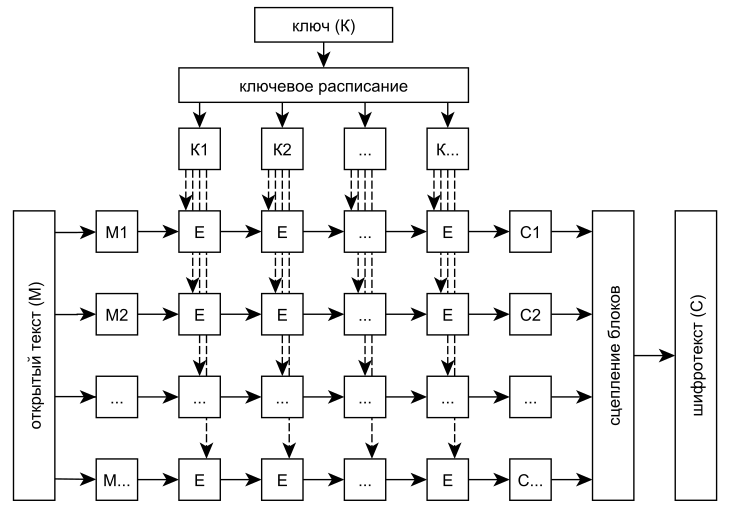
\includegraphics[width=0.8\textwidth]{block-cipher.png}
        \caption{Принцип работы блочного шифра}
    \end{figure}

    Из описания ясно, что блочные алгоритмы имеют несколько точек кастомизации:
    \begin{itemize}
        \item Размер блока
        \item Размер ключа
        \item Число раундов
        \item Функция расписания ключей
        \item Функция сцепления блоков
        \item Раундовая функция
    \end{itemize}

    Размер блока принято выбирать равным степени двойки. Как пишут авторы шифра CAST \cite{cast},
    размер блока должен быть достаточно велик, чтобы препятствовать атаке, основанной на парадоксе
    дней рождения, и не настолько большим, чтобы значительно усложнить реализацию (в том числе в
    железе). Именно поэтому в действительности вопрос выбора размера блока не представляет большого
    интереса, и многие современные шифры используют блоки в 64 или 128 битов. Так, например,
    алгоритмы DES, ГОСТ 28147-89, RC2, Blowfish и CAST, о котором речь пойдёт далее, применяют
    64-битные блоки, а алгоритмы "Кузнечик"\ и AES -- 128-битные.

    Аналогичная ситуация имеет место и с размером ключа. В приведённых выше алгоритмах длина ключа
    варьируется от 40 (CAST) до 448 битов (Blowfish). Такие алгоритмы как Blowfish позиционируются
    как шифры с переменной длиной ключа.

    Вопрос выбора функций расписания ключей и сцепления блоков представляет отдельный интерес, но
    в данной работе окажется нерассмотренным.

    Как удалось выяснить автору, бент-функциям было найдено применение в алгоритмах раундовой
    функции.

\section{Шифр CAST и применение в нём бент-функций}

    В 1997 году К.Адамсом и С.Таваресом был предложен алгоритм блочного шифрования, известный как
    CAST. Название получено из первых букв имён и фамилий авторов: Carlisle Adams, Stafford Tavares.
    Рассмотрим детально раундовую функцию алгоритма.

    \begin{wrapfigure}{r}{0.25\textwidth}
        \centering
        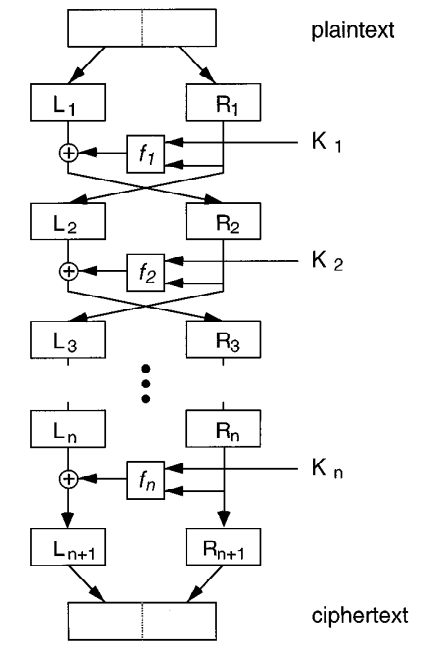
\includegraphics[width=0.25\textwidth]{feistel.png}
        \caption{Цепь ячеек Фейстеля}
    \end{wrapfigure}

    Каждый раунд в алгоритме CAST сводится к применению ячейки Фейстеля. Это очень простая
    конструкция, состоящая из двух этапов. Первый принимает на вход блок длиной $2n$ битов и
    разбивает его на две равные части: L и R. Поэтому вход ячейки Фейстеля принято сразу записывать
    в виде $(L, R)$. Выходом первого этапа является блок $(L \oplus F_i(K_i, R), R)$, где $F_i$ --
    некоторая функция, зависящая от раунда, $K_i$ -- итерационный ключ. Второй этап заключается в
    том, что левая и правая части блока после первого этапа меняются местами. Таким образом, ячейка
    Фейстеля -- отображение
    \begin{equation*}
        (L, R) \to (R, L \oplus F(K_i, R))
    \end{equation*}

    Ячейка Фейстеля последнего раунда в алгоритме CAST не выполняет перестановку левой и правой
    частей.

    Теперь рассмотрим реализацию функций $F_i$ в шифре CAST, но для этого потребуется ввести новое
    понятие.

    \textbf{Определение:} \textit{S-блоком} (блоком подстановок) называется нелинейная булева
    вектор-функция:
    \begin{equation*}
        S: \mathbb{Z}_2^m \to \mathbb{Z}_2^n
    \end{equation*}

    Под размером $S$-блока понимаем число аргументов и размерность результата.

    Любую вектор-функцию, возвращающую $n$-мерный результат, можно представить как $n$ функций
    (компонентов), возвращающих одномерный результат. Учитывая это замечание, введём также ещё одно
    понятие.

    \textbf{Определение:} \textit{идеальным} называется $S$-блок, компоненты которого являются
    бент-функциями, а также любая линейная комбинация выходных битов является бент-функцией от
    входных.

    Шифр CAST использует 4 $S$-блока размером $8 \times 32$ битов. Размер блока данных в шифре,
    составляет 64 бита. Учитывая описанную выше схему работы ячейки Фейстеля, понимаем, что на вход
    функции $F_i$ приходит 32 бита блока открытого текста.

    \begin{wrapfigure}{r}{0.3\textwidth}
        \centering
        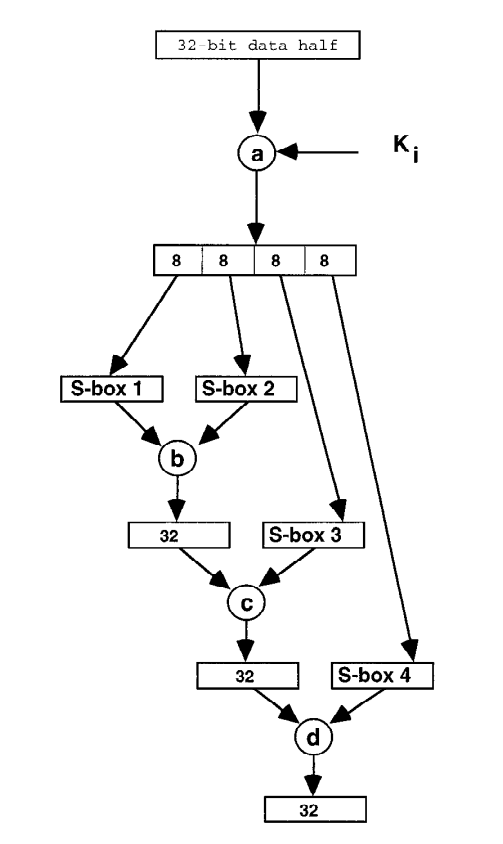
\includegraphics[width=0.3\textwidth]{round-func.png}
        \caption{Функция $F_i$}
    \end{wrapfigure}

    Алгоритм, описывающий действие функции $F_i$ следующий:
    \begin{enumerate}
        \item 32-битное число и итерационный ключ $K_i$ поступают на вход операции \textbf{a},
              возвращающей 32 бита.
        \item Результат операции \textbf{a} делится на 4 равные части по 8 битов.
        \item Каждая 8-битная часть поступает на вход одного из $S$-блоков размером
              $8 \times 32$ битов: $S_1$, $S_2$, $S_3$ и $S_4$; в результате получаем 4 32-битных
              значения.
        \item Значения, полученные от блоков $S_1$ и $S_2$, поступают на вход операции \textbf{b},
              возвращающей 32-битное значение.
        \item Значение, полученное на предыдущем шаге, и значение, полученное от блока $S_3$,
              поступают на вход операции \textbf{c}, возвращающей 32-битное значение.
        \item Значение, полученное на предыдущем шаге, и значение, полученное от блока $S_4$,
              поступают на вход операции \textbf{d}, возвращающей 32-битное значение, являющее
              возвращающим значением функции $F_i$.
    \end{enumerate}

    Как отмечают авторы алгоритма \cite{cast}, все операции \textbf{a}, \textbf{b}, \textbf{c} и
    \textbf{d} являются операцией XOR, хотя могут быть заменены и на более сложные функции.

    Итак, раундовая функция шифра CAST подробно описана. Осталось лишь выяснить, как бент-фукнции
    влияют на свойства $S$-блоков и как это отражается на свойствах раундовой функции.

\newpage
\printbibliography[heading=bibintoc, title={Список литературы}]

\end{document}
